\chapter{Methods}
\label{chapter:methods}
This chapter discusses the mathematical techniques used in this thesis. The main theories discussed here are firstly, concepts of nodal and hierarchical basis for a function representation in multidimensional spaces and consequently based on hierarchical bases theories of sparse grids and combination techniques. Respectively, these main methods construct an image about mathematical reasoning behind methods used in this thesis.

\section{Concept of nodal basis}
First idea about nodal basis comes form the finite element method and it's splitting of function into a space. The function representation in that space can be done based on nodal basis which are set of functions existing in the space. For the mathematical representation of the nodal basis, the hierarchical basis and the sparse grids, work of Garcke \cite{Garcke2013} has been used. Following same notation, let's consider a multi-index $\underline{l} = (l_{1}, \dots, l_{d}) \in \mathbb{N}^{d}$ and an anisotropic grid $\Omega_{\underline{l}}$ with mesh size $h_{\underline{l}} := \left( h_{l_{1}}, \dots, h_{l_{d}}  \right) = 2^{-l} := \left( 2^{-l_{1}}, \dots, 2^{-l_{d}} \right)$.
$\Omega_{\underline{l}}$ contains equidistant but different $h_{l_{t}}$ in coordinate direction $t, t = 1,\dots,d$ . Thus grid $\Omega$ consists of points

%equation1 
\begin{equation}
    x_{l,j} := (x_{l_{1},j_{1}}, \dots ,x_{l_{d},j_{d}})
\end{equation}
where \( x_{l_{t},j_{t}} := j_{t}\cdot 2^{-l_{t}}\) and \( j = 0,\dots,2^{l_{t}} \). An associated space $V_{\underline{l}}$ of piecewise n-linear function can be defined as  

%equation2
\begin{equation}
    V_{\underline{l}} := span\left\{\phi_{\underline{l},\underline{j}}| j_{t} = 0,\dots,2^{l_{t}} , t = 1,\dots,d \right\} = span\left\{\phi_{\underline{l},\underline{j}}| 0 \leq \underline{j} \leq 2^{\underline{l}} \right\}
\end{equation}

%equation3
\begin{equation}
    \phi_{\underline{l},\underline{j}} ( \underline{x} ) := \prod\limits_{t=1}^d \phi_{l_{t},j_{t}}(x_{t})
\end{equation}
The one dimensional functions $\phi_{l,j}$ have support
%equation4
\begin{equation}
    \left[ x_{l,j} - h_{l}, x_{l,j} + h_{l} \right] \cap [0,1] = \left[ (j-1)h_{l}, (j+1)h_{l} \right] \cap [0,1]
\end{equation}
These one dimensional functions are defined by :
%equation5
\begin{equation}
     \phi_{l,j} (x) =
     \begin{cases}
     1 - \left|x/h_{l} - j \right|, &  x \in \left[ (j-1)h_{l}, (j+1)h_{l} \right] \cap [0,1] \\
     0, & \text{otherwise}
     \end{cases}
\end{equation}
This representation is basically a representation on nodal basis.
\section{Concept of hierarchical basis}
The conversion of the function coefficients on a grid from standard nodal basis to the representation in hierarchical basis is carried out by a constant operation count per grid point. The transformation to the hierarchical basis representation is done by the algorithm described thoroughly in \cite{Griebel1992b} which gives us further insight into the hierarchical basis.  So, after defining the multi-indices, space, grids and one dimensional basis functions, one needs to define hierarchical difference space $W_{\underline{l}}$
%equation6
\begin{equation}
     W_{\underline{l}} := V_{\underline{l}} \setminus \bigoplus\limits_{t=1}^{d} V_{\underline{l}} - \underline{e}_{t}
\end{equation}

where $\underline{e}_{t}$ is the t-th unit vector. From the definition of the index set
%equation7 --- here I have taken liberty of conveying the information slightly differently
\begin{equation}
     \phi_{l,j} (x) =
     \begin{cases}
     j_{t} = 1,\dots,2^{l_{t}} -1, &  j_{t} \text{ odd }, t= 1,\dots,d, \text{ if } l_{t} > 0\\
     j_{t} = 0,1,, & t=1,\dots,d \text{ if } l_{t} = 0 
     \end{cases}
\end{equation}
It leads to 

%equation8
\begin{equation}
     W_{\underline{l}} = span\left\{\phi_{\underline{l},\underline{j}} | \underline{j} \in \text{ B}_{\underline{l}}\right\}
\end{equation}

The hierarchical difference spaces leads us to multilevel subspace decomposition. We can write the spaces as the direct sum of the subspaces
%equation9
\begin{equation}
     V_{n} := \bigoplus\limits_{l_{1} = 0}^n \dots \bigoplus\limits_{l_{n} = 0}^n W_{\underline{l}} = \bigoplus\limits_{\left|\underline{l} \right|_{\infty} \leq n} W_{\underline{l}}
     \label{eq9}
\end{equation}
where
%equation10
\begin{equation}
     \left|\underline{l} \right|_{\infty} := \text{ max}_{1 \leq t \leq n} l_{t} \text{ and } \left|\underline{l} \right|_{1} := \sum\limits_{t=1}^{n} l_{t}
\end{equation}
The set of functions
%equation11
\begin{equation}
     \left\{phi_{\underline{l},\underline{j}} | \underline{j} \in \text{ B}_{\underline{l}} \right\}_{\underline{l} = \underline{0}}^{\underline{n}}
\end{equation}
is hierarchical basis of $V_{n}$. Therefore, every function $f \in V_{n}$ can be represented as
%equation12 
\begin{equation}
	f(\underline{x}) = \sum_{|\underline{l}|_\infty\le n} \sum_{|\underline{j}| \in \text{B}_{\underline{l}}} \alpha_{\underline{l},\underline{j}} \cdot \phi_{\underline{l},\underline{j}} (x) = \sum_{|\underline{l}|_\infty\le n} f_{\underline{l}}(\underline{x}), \quad \text{with} \ \ f_{\underline{l}} \in W_{\underline{l}}
\end{equation}

where $\alpha_{\underline{l},\underline{j}} \in \mathbb{R} $
are the coefficients of the representation in the hierarchical tensor product basis. 

Furthermore,
%equation13 
\begin{equation}
    V := \lim\limits_{n\rightarrow\infty} \bigoplus_{|\underline{k}|\le n} W_{\underline{k}}
\end{equation}

The generalized d-dimensional hierarchization operator can be written as
%equation14 
\begin{equation}
    \alpha_{\underline{l},\underline{j}} = \left( \prod_{t=1}^{n}
    \left[
    \begin{array}{ccc}
	    -\dfrac{1}{2} & 1 & -\dfrac{1}{2}
    \end{array}
    \right]_{l_t,j_t}
     \right) f
\end{equation}
The hierarchical basis simplifies the calculations with the functions that are defined in different grids. As an example, one can simply add the single coefficients for calculation the addition of two functions that are defined the different grids, because basis functions associated with the same grid points are exactly same\cite{Griebel1992b}.\\
Note that, with a cursory glance, the hierarchical matrices seems complicated however one needs to factorize the matrices into the general nodal basis stiffness matrix and sparse matrices. It is not required to assemble the discretization matrix.\cite{Yserentant1986}. 
Comparison of nodal and hierarchical basis for one dimensional level three has been shown in figure. \ref{fig:NodalHierBasisLevel3}.

\begin{figure}[h]
	\centering
    \begin{subfigure}[b]{0.49\textwidth}
	    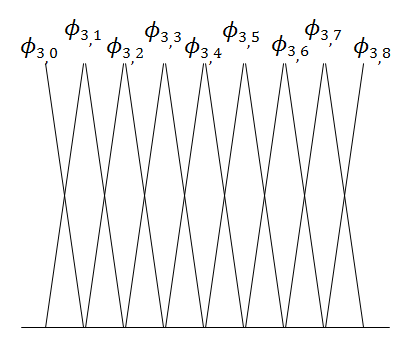
\includegraphics[width =\textwidth]{/NodalBasisLevel3.png}
	    %\vspace{3em}
		\centering
        \caption{Nodal basis}
    \end{subfigure} 
    \begin{subfigure}[b]{0.49\textwidth}    
	    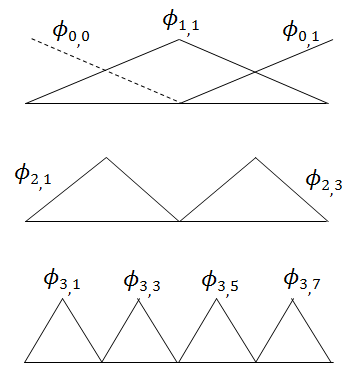
\includegraphics[width =\textwidth]{/HierBasisLevel3.png}
		\centering    
	 \caption{Hierarchical basis}
    \end{subfigure} 
    \caption{Nodal and hierarchical basis of level $n=3$. }
    \label{fig:NodalHierBasisLevel3}
\end{figure}		

\section{Sparse Grids based on hierarchical subspace splitting}
 Efficient discretization techniques are imperative for majority of problems in numerical mathematics such as interpolation, point approximation etc. Introduced by Zenger in \cite{Zenger1990} and based on hierarchical tensor product approximation spaces, sparse grids provide an efficient approach to improve the ratio of invested storage and computing time to the achieved accuracy.\cite{Bungartz1998}\\
  Following \cite{Zenger1990} finite element space is the direct sum of the subspaces where the error propagation is equal or larger than some prescribed tolerance. This leads to an approximation space that corresponds to a sparse grid in place of a full grid.\\
Hierarchical basis functions with small support and small contribution to function representation are not included in discrete space level n .This type of grids are classisified as sparse grids. 
%equation15 
\begin{equation}
    V_{n}^s := \bigoplus_{|\underline{l}|_1\le n} W_{\underline{l}}
\end{equation}
Using \eqref{eq9}, we get 
%equation16
\begin{equation}
    f_{n}^s \left(\underline{x}\right) 
    = \sum_{|\underline{l}|_1\le n} \sum_{|\underline{j}|\in B_{\underline{l}}} \alpha_{\underline{l},\underline{j}}\phi_{\underline{l},\underline{j}}\left(\underline{x}\right) 
    = \sum_{|\underline{l}|_1\le n} f_{\underline{l}}(\underline{x}), \quad \text{with} \ f_{\underline{l}} \in W_{\underline{l}}
\end{equation}

The sparse grids can also be formulated as follows:
%equation17
\begin{equation}
    V_{0,n}^s := \bigoplus_{|\underline{l}|_1\le n+d-1} W_{\underline{l}}, \quad l_t > 0
\end{equation}

The approximation error can defined as
%equation18
\begin{equation}
	\parallel f - f_{0,n}^s \parallel \le \sum_{|\underline{l}|_1\le n+d-1} \parallel f_{\underline{l}}\parallel
\end{equation}

where as the interpolation error is defined as 
%equation19
\begin{equation}
	{\parallel f - f_{n}^s \parallel}_{2} = \mathcal{O}\left(h_n^2\log{}(h_{n}^{-1})^{d-1} \right)
\end{equation}

\section{Combination technique}
To discretize a function $f$ on particular combination of anisotropic grids $\Omega_{\underline{l}}$ with uniform mesh size $h_{t} = 2^{l_{t}}$ in the t-th coordinate direction.  different grids have different mesh sizes for different directions. 
all grids can be considered with
%equation20
\begin{equation}
	|\underline{l}| := l_1 + ... + l_d = n-q, \ \ q = 0,...,d - 1, \ \ l_t \ge 0
\end{equation}

Using finite element approach with piece-wise linear function in each dimensions, one gets the nodal basis as discrete partial functions from different grids using the combination formula
%equation21
\begin{equation}
	f_n^c(\underline{x}) := \sum_{q=0}^{d-1}(-1)^q \left( \begin{array}{c}
	d-1 \\
	q  \end{array} \right) \sum_{|\underline{l}|_1=n-q} f_{\underline{l}}(\underline{x})
\end{equation}
The function $f_n^c(\underline{x})$ is a part of the sparse grid scpace $V_{n}$ .
%equation22
\begin{equation}
	|f-f_n^c| = \mathcal{O}\left(h_n^2 \cdot \log(h_{n}^{d-1}) \right)
\end{equation}

One can also consider ANOVA representation in form the combination method, where the function can be represented as
%equation23
\begin{equation}
	f(\underline{x}) = \sum_{\{j_1,...,j_q\}\subset\{1,...,d\}} c_{j_1,...,j_q} f_{j_1,...,j_q} \left( x_{j_1},...,x_{j_q} \right)
\end{equation}
where each $f$ depends only depends only on a subset of size $q$ of the dimensions. It is also possible that there exist different refinement levels for each dimension. If dimension $q$ is significantly smaller than $d$, then the complexity is only dependent on $q$, which is also called superposition dimension. An advantage of such case is beneficial where one can choose grids of their own and not follow the grid sequence.. This is known as the dimension adaptive procedure. Here an index set $I$ is expressed such that one needs to fulfill an admissibility condition
%equation24
\begin{equation}
	\underline{k} \in \text{I} \ \ \text{and} \ \ \underline{j}\le \underline{k} \quad \implies \quad \underline{j}\in \text{I}
\end{equation}
It means that index $\underline{k} \in I$ if all smaller grids belong to $I$. The combination coefficients for dimension adaptive combination technique depends only upon the index set $I$. 
%equation25
\begin{equation}
    f_I^c\left(\underline{x}\right) := \sum\limits_{\underline{k} \in I}\left( \sum\limits_{\underline{z} = \underline{0}}^{1}\left(-1\right)^{\left|\underline{z}\right|1}\cdot \chi^{I}\left(\underline{k}+\underline{z}\right)\right)f_{k}\left(x\right)
\end{equation}
where $\chi^{I}$ is the characteristic function of I and is expressed as follows
%equation 26
\begin{equation}
     \chi^{I}(\underline{k}) =
     \begin{cases}
        1 &  \text{ if } k \in I\\
        0 & otherwise 
     \end{cases}
\end{equation}

\section{Combination Technique}
Another motivation for sparse grids is to represent any sparse grid function as a linear combination of its interpolants on the regular full grids. This requires us to seek a certain linear combination of full grid spaces to create a sparse grid space. This approach do away with the need for data structures more complicated than a few arrays to store a sparse grid function and requires only regular data structures.\cite{Griebel1992b} \\
The crux of the combination technique is similar to the multilevel splitting of the finite element spaces which changes the nodal bases of the space with hierarchical bases. \cite{Yserentant1986} The basis for combination techniques comes from the liner combination of independent solution of many problems with reduced size. \cite{Griebel1992}. Figure \ref{fig:Sparsegrid} shows an example of this multilevel combination which is basically addition and subtraction in this special case.

		\begin{figure}
			\centering
			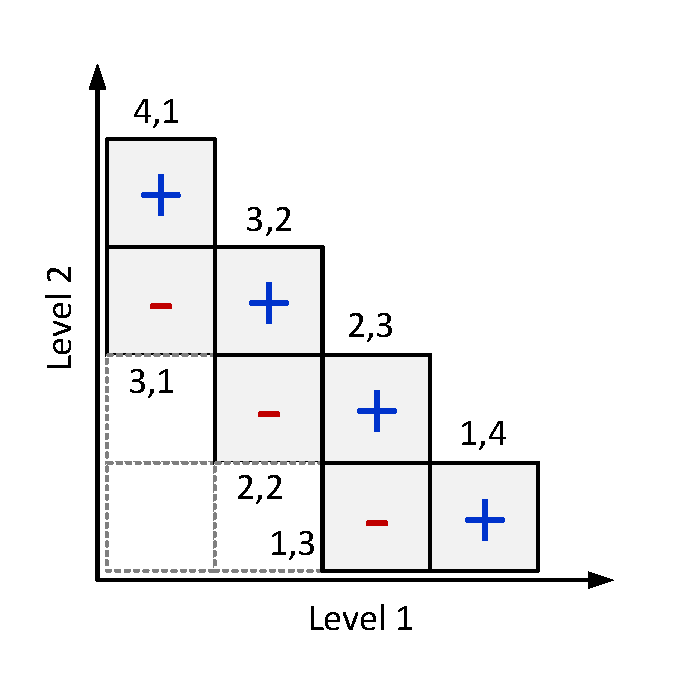
\includegraphics[width=0.6\textwidth]{/SparseGrid.pdf}
			\caption{Classical sparse grid combination method for l=4}
			\label{fig:Sparsegrid}
		\end{figure}

In total combination technique involves $O({h}^{-1}_nlog({h}^{-1}_n))$  unknowns in contrast to $O({h}^{-2}_n) $ unknowns for the conventional full grid approach however combination solution is nearly as accurate as the standard solution. it can be proven that error is only slightly worse than for the associated full grid.\cite{Griebel1992a, Griebel1992b}. To some extent the combination technique even works for non-smooth solutions. Now, ${h}^2_i$ and ${h}^2_j$ in have to be replaced by ${h}^\alpha_i$ , ${h}^\beta_j$ with appropriate $\alpha$ and $\beta$, but because of the properties of the combination technique the leading error terms still cancel. However, for the problems with severe singularities, the appropriate combination of adaptively refined grids is recommended.\cite{Griebel1992a}\\ It is seen that in some situations the combination technique leads to the cancellation of certain error terms in the asymptotic error expansion\cite{Griebel1992b} \\
 Lastly, one should note that the error analysis of this method has been relatively explained in \cite{Garcke2013} and the references there within. For further details please check the chapters of related works under "Works on Error Analysis and Convergence" presented earlier in the thesis. The discussion of these analysis is out of scope for this thesis but perhaps relatively important in future works.
%
%\section{Some General Discussions and Points}
%1. The resulting algorithm can be used as a solver and within a preconditioner. it can also be applied as a preconditioner for the full grid problem to speed up a basic iterative solver. \cite{Griebel1992} \\
%
%\subsection{Argument of error and convergence}
%1. We show that the condition number of such a stiffness matrix for multilevel splitting of finite element spaces behaves like $O((log \kappa)^2) $ where $\kappa$ is the condition number of the stiffness matrix with respect to a nodal basis. \cite{Yserentant1986} \\
%2. error satisfies $O({h}^2_nlog({h}^{-1}_n))$ (pointwise and with respect to the $L_2$- and $L_\infty$-norm).\cite{Griebel1992b} \\
%
%3. For the Poisson equation on the unit square it is proved that the combined solution converges with order $O(h)$ in the energy norm and with order $O(h^2log h)$ in the $L^2$-norm. (journals 5 and 9 are very similar aka poisson vs. second-order elliptic differential equations-9 general of 5) \cite{Pflaum1993}\\
%
%\subsection{Argument of Preconditioner plus solver}
%1. The resulting algorithm can be used as a solver and within a preconditioner. it can also be applied as a preconditioner for the full grid problem to speed up a basic iterative solver. \cite{Griebel1992} \\
%
%2. In addition to being a solver in its own right, the combination method can be used as a parallel preconditioner for the full grid problem. Then, a basic iterative method is accelerated substantially and shows nearly optimal, i.e. multigrid-like convergence behavior, if the accuracy of the solution is required only up to the truncation error.\cite{Griebel1992} \\
%
%\subsection{Argument of relation between hierarchical basis and nodal basis}
%1. As the representation of a finite element function with respect to a hierarchical basis can be converted very easily and quickly to its representation with respect to a nodal basis, our results mean that the method of conjugate gradients needs only logarithm of the dimension of the finite element space steps and computer operations to reduce the energy norm of the error by a given factor if one uses hierarchical bases or related preconditioning procedures. \cite{Yserentant1986} \\
%
%2.Two dimensional sparse grids contain only $O({h}^{-1}log({h}^{-1}))$ grid points in contrast to the usually used full $O({h}^{-2}) $ grids, whereas for a sufficiently smooth function the accuracy of the representation is only slightly deteriorated. from $O(h^2) $ to $O(h^{2}log({h}^{-1}))$. \cite{Griebel1992b} \\
%
%3. Using this type of hierarchical basis the calculation with functions defined on different grids and spaces is simplified. For example, the addition of two functions defined on different grids is reduced to the addition of the single coefficients. This is due to the fact that now the basis functions that are associated with the grid points which belong to both grids are just the same. \cite{Griebel1992b} \\
%
%4. The transformation of the coefficients of a function on grid represented in standard nodal basis to its representation in hierarchical basis can be implemented by a constant number of operations per grid point. The transformation to the hierarchical basis representation is done by the algorithm in \cite{Griebel1992b}. \\
%
%5. The advantage of using the hierarchical basis representation during the combination process is that no interpolation to additional grid points has to be performed explicitly: For each 'missing' grid point, the interpolated value would be zero in hierarchical basis representation, and thus can be omitted during the combination of solutions\cite{Griebel1995} \\
%
%6. One of the main advantages of hierarchical bases compared with standard nodal point bases is probably the fact that the basis gets a multilevel structure. Thus, we can now distinguish between high-level basis functions with a large support that usually (in the smooth case, at least) already contain a significant part of the information, and functions living on lower levels whose contribution to an interpolant or a finite element approximation is rather small. The decrease of the hierarchical coefficients from level to level can be used, of course, to control adaptive grid refinement, but, if it is combined with a tensor product approach for the higher dimensional case, it can be used for an a priori reduction of the number of grid points involved in the calculation, too.\cite{Bungartz1998}\\
%
%7. The hierarchical coefficient or hierarchical surplus itself can be used to indicate the smoothness of u at the corresponding grid point and, consequently, the necessity to refine the grid here.\cite{Bungartz1998}\\
%
%8. The elements of the sparse grid space can be represented in a hierarchical basis [27] and many algorithms for hierarchical basis methods including wavelets can be used for the solution [5,20]. Compared to the commonly used nodal basis, a hierarchical basis of, e.g. multilinear functions has its disadvantages, as the corresponding matrices have reduced sparsity and a less regular structure. This is due to the fact that the supports of the lower level basis functions are large and intersect nontrivially with many higher level basis functions. These difficulties increase with dimension.
%An efficient way to avoid the problem of reduced sparsity is given by the combination technique. \cite{Hegland2007}\\
